\documentclass{beamer}
\mode<presentation>
{
  \usetheme{default}      % or try Darmstadt, Madrid, Warsaw, ...
  \usecolortheme{default} % or try albatross, beaver, crane, ...
  \usefonttheme{default}  % or try serif, structurebold, ...
  \setbeamertemplate{navigation symbols}{}
  \setbeamertemplate{caption}[numbered]
} 

\usepackage[english]{babel}
\usepackage[utf8x]{inputenc}
\usepackage{scrextend}
\usepackage{graphicx}
\usepackage{booktabs}
\usepackage{adjustbox}
\usepackage{marvosym}
\graphicspath{ {E:/images/} }

\title[Pres]{Dezvoltarea de metode de analiză automată a sistemelor software}
\author{Student : Stana Adelina Diana\\Conducător stiințific :  prof.dr.ing. Vladimir Crețu}
\institute{Departamentul Calculatoare şi Tehnologia Informaţiei\\
Universitatea Politehnica Timișoara}
\date{Iulie, 2018}

\begin{document}

\begin{frame}
  \titlepage
\end{frame}

% Uncomment these lines for an automatically generated outline.
%\begin{frame}{Outline}
%  \tableofcontents
%\end{frame}
%%%%%%%%%%%%%%%%%%%%%%%%%%%%%%%%%%%%%%%%%%
 \begin{frame}
\frametitle{Cuprins}

\begin{itemize}
\item Direcțiile și intențiile de studiu avute în vedere pentru programul doctoral.
\item Concordanța dintre domeniul de doctorat si pregătirea anterioară.
\item Gradul de inițiere:
\begin{itemize}
\item in activitati practice
\item in activitati de cercetare
\end{itemize}
\item Lucrări stiințifice publicate sau comunicate cu tematică asociată domeniului de doctorat.
\end{itemize}

\end{frame}

%%%%%%%%%%%%%%%%%%%%%%%%%%%%%%%%%%%%%%%%%%
 \begin{frame}
\frametitle{Direcțiile și intențiile de studiu avute în vedere pentru programul doctoral}

\begin{itemize}
\item investigarea a noi metode de rafinare/filtrare a dependențelor logice extrase din modul de evoluție a sistemelor software.
\item  investigarea în ce măsură informațiile aduse de dependențele logice aduc îmbunătățiri ale metodelor de reconstrucție arhitecturală:
\begin{itemize}
\item reclusterizare
\item identificare a modulelor arhitecturale importante
\end{itemize}
\end{itemize}

\end{frame}
%%%%%%%%%%%%%%%%%%%%%%%%%%%%%%%%%%%%%%%%%%

 \begin{frame}
\frametitle{Pregătirea anterioară}

Studiile absolvite pană in prezent sunt:\\
- \textbf{Licența} la facultatea de Automatică și Calculatoare, UPT, in domeniul CTI, specializarea Calculatoare, cu opționale pe pachetul de Software Engineering, media de absolvire 8,87.

Tema lucrarii de licenta a fost \textit{“Sistem distribuit pentru gestionarea interacțiunii clienților cu sistemul de versionare.”} obtinând nota 9,66  în sesiunea Iunie 2016.

- \textbf{Master} la facultatea de Automatică și Calculatoare, UPT, in domeniul CTI, specializarea Information Technology, media de absolvire 9,75. 

Tema lucrarii de dizertatie a fost \textit{“An analysis of the relationship between structural and logical dependencies in software systems.”} obtinând nota 10 în sesiunea Iunie 2018.

\end{frame}

%%%%%%%%%%%%%%%%%%%%%%%%%%%%%%%%%%%%%%%%%%%
 \begin{frame}
\frametitle{Gradul de inițiere în activități practice}
\begin{block}{}
La locul de muncă de la Continental ca software developer (4 ani). 
\end{block}
\begin{itemize}
\item limbaje de programare: Python, C++, C\#
\item medii de dezvoltare: Visual Studio, PyCharm
\item sisteme de versionare : SVN, Git
\end{itemize}


\end{frame}

%%%%%%%%%%%%%%%%%%%%%%%%%%%%%%%%%%%%%%%%%%%

 \begin{frame}
\frametitle{Gradul de inițiere în activități de cercetare}
\begin{block}{}
Lucrarea de disertație: “An analysis of the relationship between structural and logical dependencies in software systems.”
\end{block}

\begin{center}
     \begin{figure}
	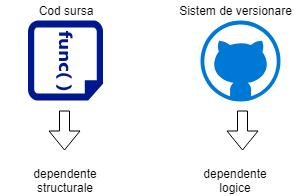
\includegraphics[width=3in]{dep.png}
	\caption{\label{fig:figtool} Dependențe logice și structurale}
     \end{figure}
\end{center}
\end{frame}

%%%%%%%%%%%%%%%%%%%%%%%%%%%%%%%%%%%%%%%%%%%

 \begin{frame}
\frametitle{Tool pentru extragerea dependențelor }
Am construit un tool de analiză pentru extragerea ambelor tipuri de dependențe software.  
\begin{center}
     \begin{figure}
	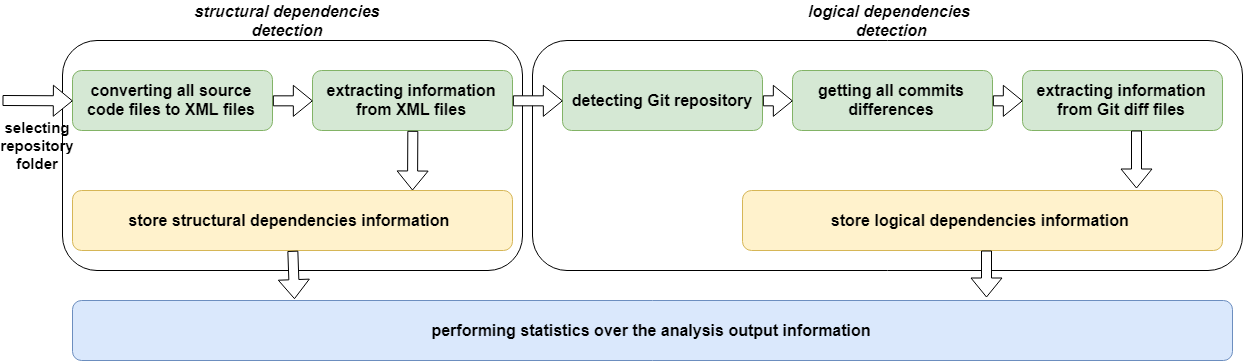
\includegraphics[width=\textwidth]{fig3.png}
	\caption{\label{fig:figtool} Tool workflow}
     \end{figure}
\end{center}

\end{frame}

%%%%%%%%%%%%%%%%%%%%%%%%%%%%%%%%%%%%%%%%%%%

 \begin{frame}
\frametitle{Metode de filtrare ale dependențelor logice}
Dependențele logice au fost extrase în funcție de următoarele filtre:

\begin{itemize}
\item Numărul de fișiere existente într-un commit. Valorile pentru acest filtru: 5, 10, 20 și fără limită de fișiere.
\item Numărul de apariții a unei dependente logice. Valorile pentru acest filtru: 1, 2, 3 și 4 apariții.
\item Cu/fără luarea în considerare a comentariilor ca schimbări valide.
\end{itemize}

\end{frame}

%%%%%%%%%%%%%%%%%%%%%%%%%%%%%%%%%%%%%%%%%%%

 \begin{frame}
\frametitle{Rezultate}
Am studiat 17 sisteme open-source cpp si java.
\begin{center}
     \begin{figure}
	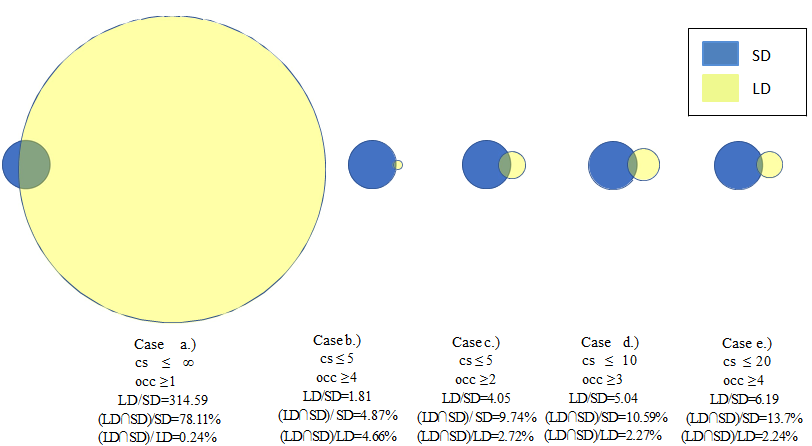
\includegraphics[width=\textwidth]{figvennpdf.png}
	\caption{\label{fig:figvenn}Relațiile între dependențele logice și structurale pentru diferite variante de filtre. }
     \end{figure}
\end{center}


\end{frame}

%%%%%%%%%%%%%%%%%%%%%%%%%%%%%%%%%%%%%%%%%%%

 \begin{frame}
\frametitle{Concluzii}

\begin{itemize}
\item Cea mai mare influentă asupra rezultatelor o are filtrarea după numărul de fișiere și filtrarea după numărul de apaiții a dependențelor logice.
\item Filtrele aplicate individual nu duc la filtrarea dependentelor cu adevarat logice, cea mai buna solutie pentru filtrare fiind combinarea filtrelor propuse.
\item Filtrarea comentariilor are o influență mică asupra rezultatelor finale (+-3\%).
\end{itemize}

\end{frame}

%%%%%%%%%%%%%%%%%%%%%%%%%%%%%%%%%%%%%%%%%%%

 \begin{frame}
\frametitle{Direcții de cercetare abordate la doctorat}


\begin{itemize}
\item În urma măsuratorilor aproximativ 80\% din dependentele logice nu sunt și structurale. În viitor dorim să studiem cauzele acestei diferențe mari între cele două categorii prin:
\begin{itemize}
\item Extragerea dependențelor structurale și din versiuni mai vechi ale codului, nu doar din cea mai recentă versiune.
\item Filtrarea pe baza trendului crescator sau descrescator in timp al numarului de aparitii al dependentelor logice.
\end{itemize}
 \item Utilizarea informațiilor aduse de dependențele logice în îmbunătățirea metodelor de reconstrucție arhitecturală prin combinarea lor cu dependențele structurale.
\end{itemize}
\end{frame}


%%%%%%%%%%%%%%%%%%%%%%%%%%%%%%%%%%%%%%%%%%%

 \begin{frame}
\frametitle{Lucrări stiințifice}
[1] Adelina Stana, Ioana Șora, \textit{„An analysis of the relationship between structural and logical dependencies in software systems”} trimisă la Sesiunea de Comunicări Ştiinţifice Studenţeşti UPT, comunicată.

[2] Ioana Șora, Adelina Stana, \textit{„Identifying logical dependencies from co-changing classes”}  trimisă la The 7th International Workshop on Mining Software Repositories (SOFTWAREMINING-2018) - colocated with The 33rd IEEE/ACM International  Conference on Automated Software Engineering (ASE 2018), Montpellier, Franta, Sept 2018, în așteptarea deciziei de review.


\end{frame}

%%%%%%%%%%%%%%%%%%%%%%%%%%%%%%%%%%%%%%%%%%%

 \begin{frame}
\frametitle{Lucrări stiințifice}

[3] Adelina Stana, Ioana Șora, Vladimir Crețu, \textit{„Logical dependencies between classes: how to find them and how to use them ?”} trimisă la The 34th IEEE International Conference on Software Maintenance and Evolution (ICSME) 2018 - Doctoral Symposium, Madrid, Spania, Sept 2018, lucrare acceptată.
\end{frame}



%%%%%%%%%%%%%%%%%%%%%%%%%%%%%%%%%%%%%%%%%%%

\end{document}
